\subsection{Detection and Localization}

Here, two experiments have been conducted: a real experiment in a Lake, and a simulation under more controlled conditions.

\subsubsection{Lake experiments}
We evaluated the detector on magnetic data, recorded in the lake of Bourg-Blanc, approximately 15 km northeast of Brest, in Brittany, France.

The experiment involved a USV (dimensions: 180 × 120 cm), following a predetermined path while carrying a triaxial fluxgate magnetometer, photos are shown in figure \ref{fig:experiment_setup}.

The magnetic data were acquired using an autonomous data acquisition system developed by MAPPEM Geophysics. The magnetic sensor is a 3-axis fluxgate magnetometer with a noise level of 20 pT/$\sqrt{\text{Hz}}$ at 1 Hz. The data logger is synchronized at start-up on GNSS time, and acquisition is paced by a precise oscillator with an error of about 1 s per year. The data logger records the 3 components simultaneously at 500 Hz with 32-bit resolution. For the experiment, the magnetometer was installed on the USV at a distance from major electromagnetic noise sources.

\begin{figure*}[t]
\centering
\begin{minipage}[t]{0.32\textwidth}
\centering
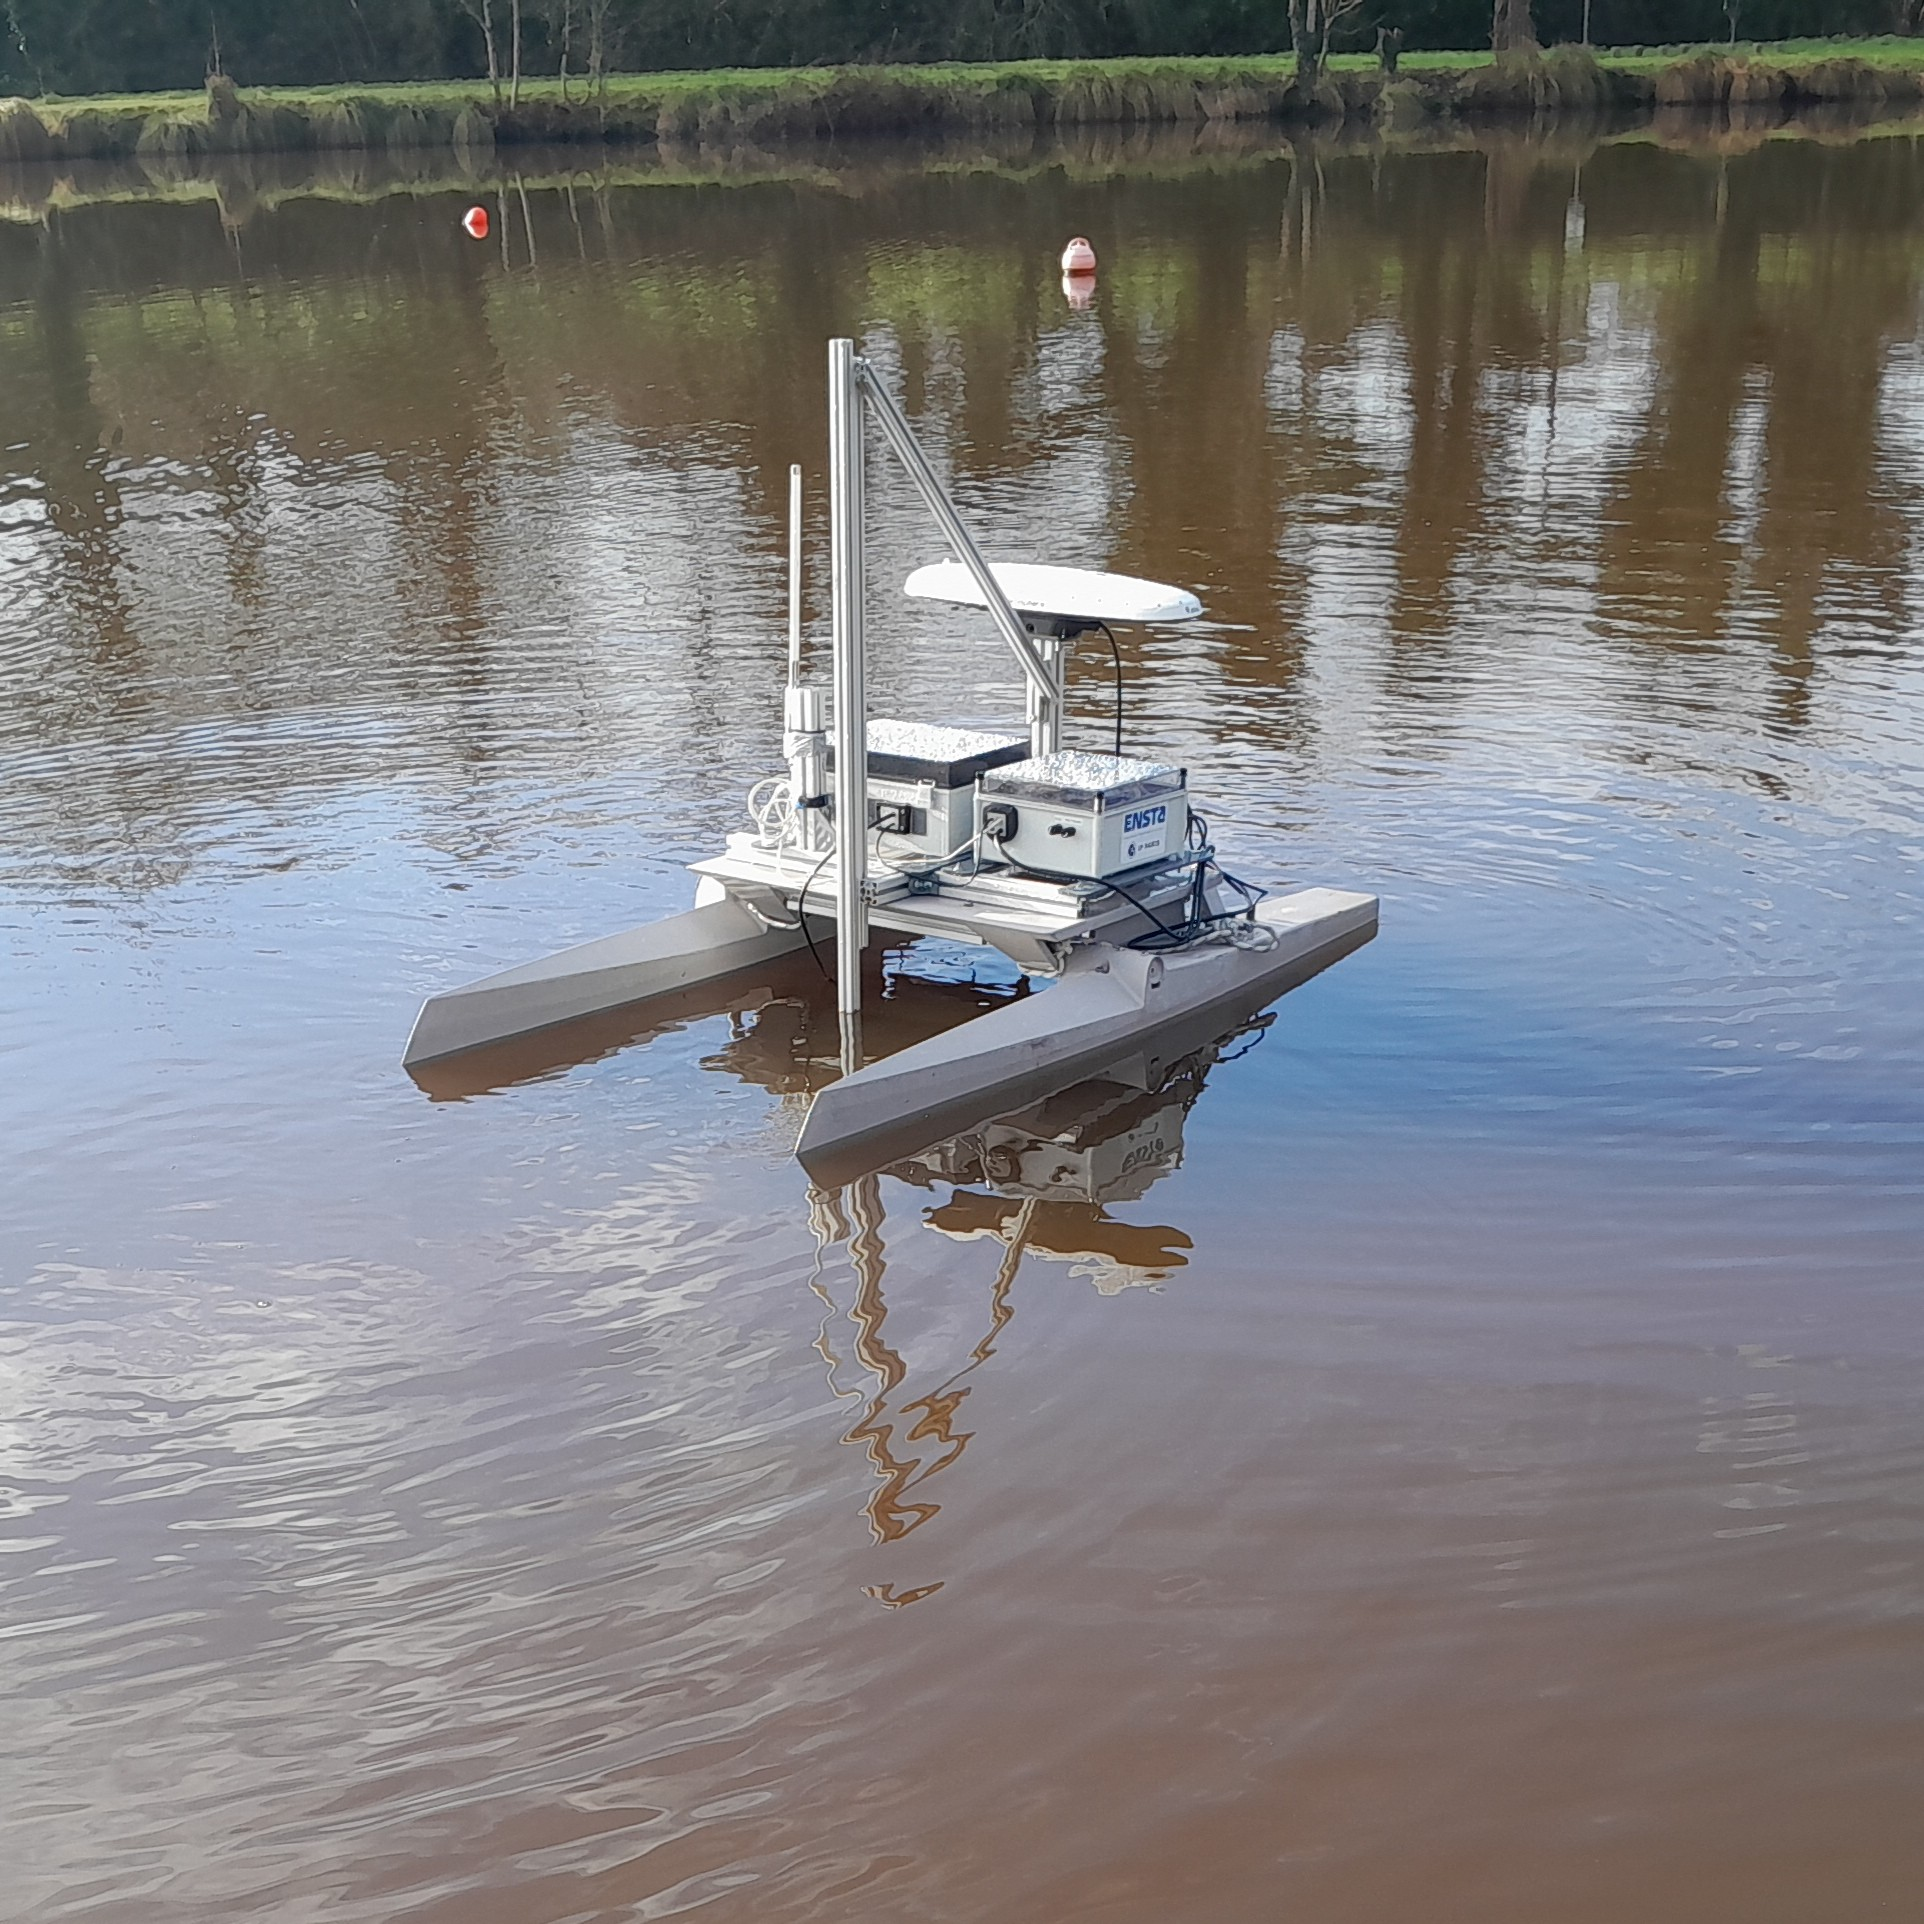
\includegraphics[width=\linewidth]{results_and_discus/figures/helios_photo.jpg}
\end{minipage}
\hfill
\begin{minipage}[t]{0.62\textwidth}
\centering
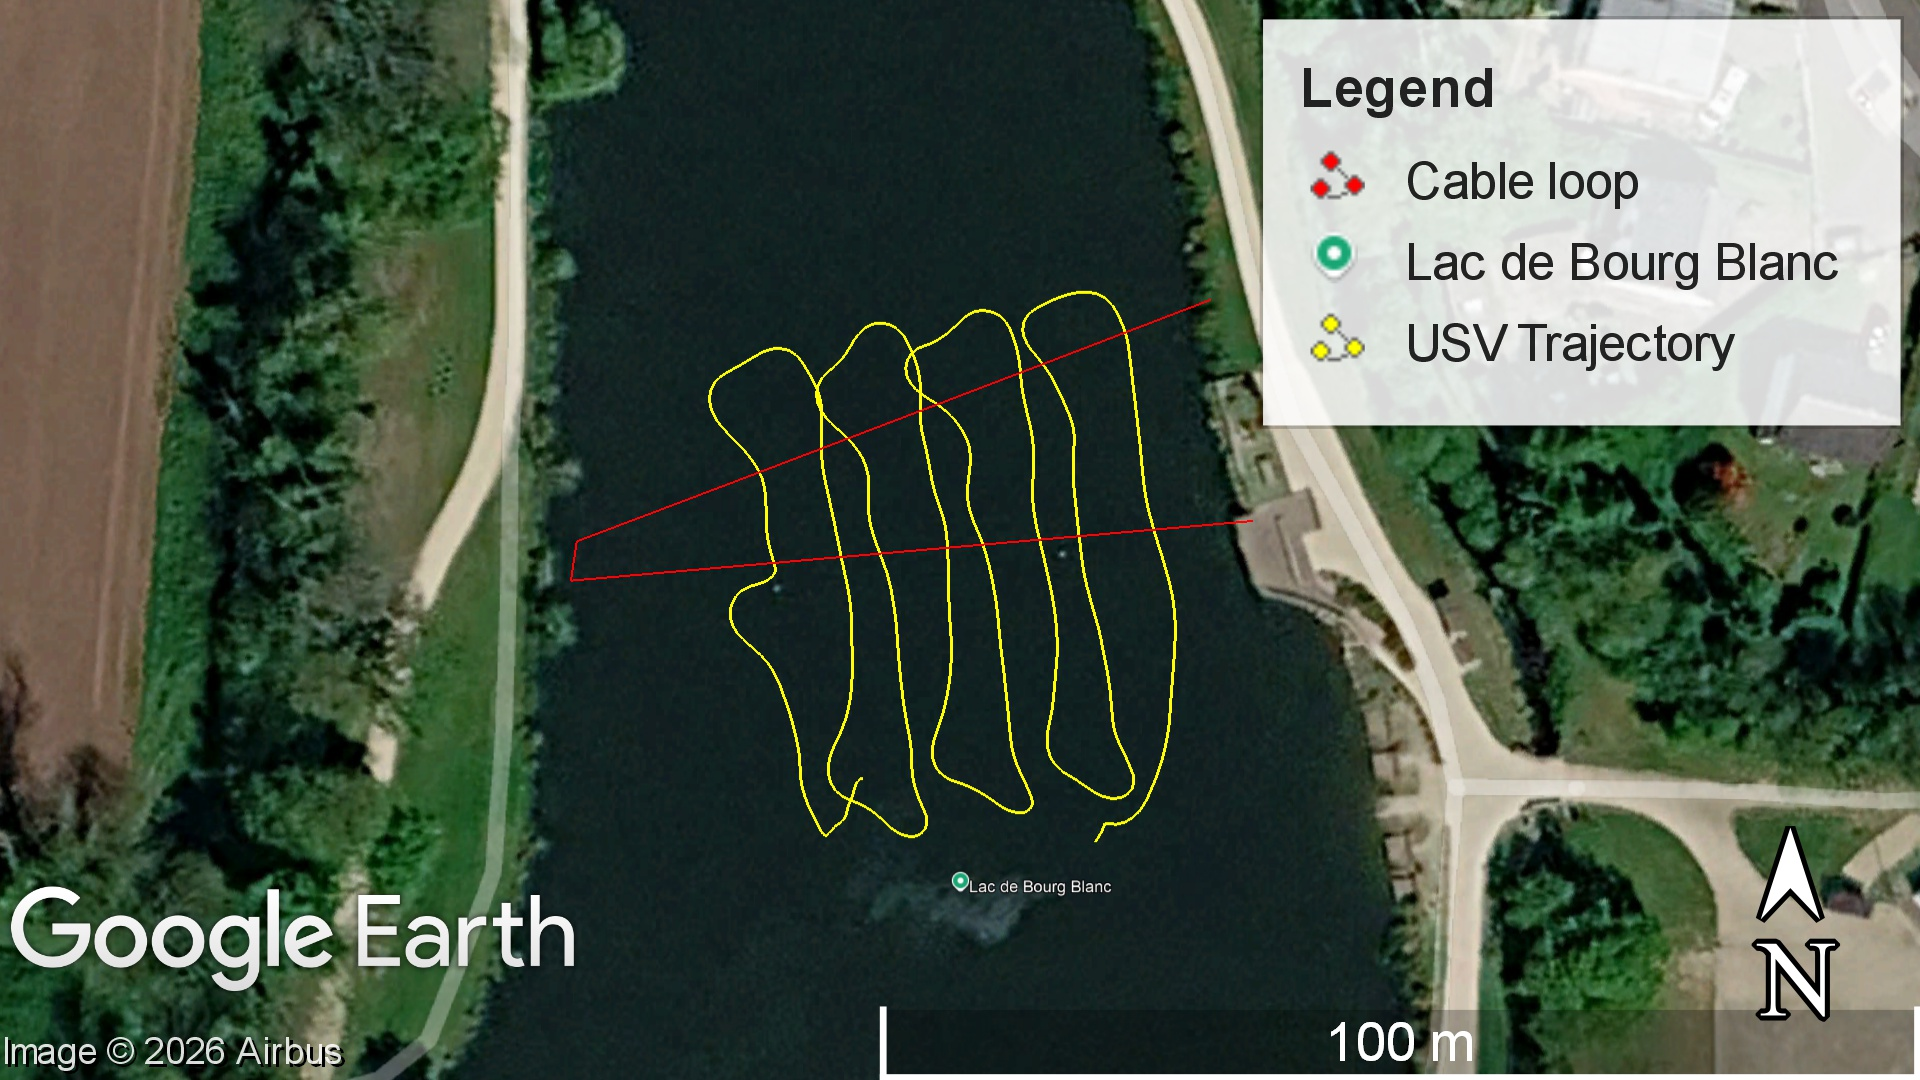
\includegraphics[width=\linewidth]{results_and_discus/figures/google_earth.jpg}
\end{minipage}
\caption{Experimental platform and test site.}
\label{fig:experiment_setup}
\end{figure*}

To set up the experiment, a loop of wire approximately 170~m long was deployed in the lake, at a depth between 1.5 and 2 meters, and energized with a DC current of 6A.
The USV was programmed to follow a lawnmower trajectory and cross the cable at a 90-degree angle with an average velocity of $0.65~m/s$.

The norm of the recorded magnetometer data was then provided as the input to the detector, as defined in Section~\ref{sec:detector}, and the filter templates—namely, the OBF—were applied over a temporal window of 32 seconds.


As a baseline, we considered MOBF of order 1 (Anderson OBF), which is the most common for dipole detection, and compared it against our cable OBF and MOBF of order 2 (dipole + quadrupole)\footnote{The order of an MOBF receiver denotes the highest multipole
retained: order~1 is the dipole (Anderson) receiver, and order~2 the
quadrupole receiver. We refer to the latter interchangeably as
``quadrupole'' (naming it by its highest retained multipole) or
``dipole~+~quadrupole'' (naming it by the source content it captures),
both designate the same order-2 receiver. These are not independent bases
stacked together, the multipolar subspaces are not in direct sum, so
order~2 is a single orthonormal set that subsumes the dipole contribution.}.

Two types of figures have been produced: first, figure \ref{fig:trajectory_comparison}, which is the drone trajectory, colored according to the measured magnetic anomaly ( $F_s - |\vec T |) $, the true cable crossing positions are marked with a star, and the detections from the filter are marked with red crosses.

A second plot, figure \ref{fig:filter_output_comparison}, represents the normalized filter input (recorded magnetic anomaly) with the normalized filter output, the crosses indicate true cable crossing moments, and the red dots represent the filter detections (which are the peaks after thresholding).


Analyzing the results, we see a clear distinction in performance: the MOBF misses the cable's exact location. In other words, the filter's maximum output lags the CPA moment by a measurable error of 1.56 and 1.9 meters for orders 1 and 2, respectively, whereas the detector based on cable OBF shows a reasonable error of 0.6 meters. 

We note that in the real experiment, part of the lag is due to localization error at the GNSS level. In Figure \ref{fig:filter_output_comparison}, we do not see isolated peaks in the filter output, and that is due to the two extremes of the cable loop being close to each other. A cleaner comparison is in the simulated experiment.


\begin{figure}[ht]
    \centering
    Cable OBF
    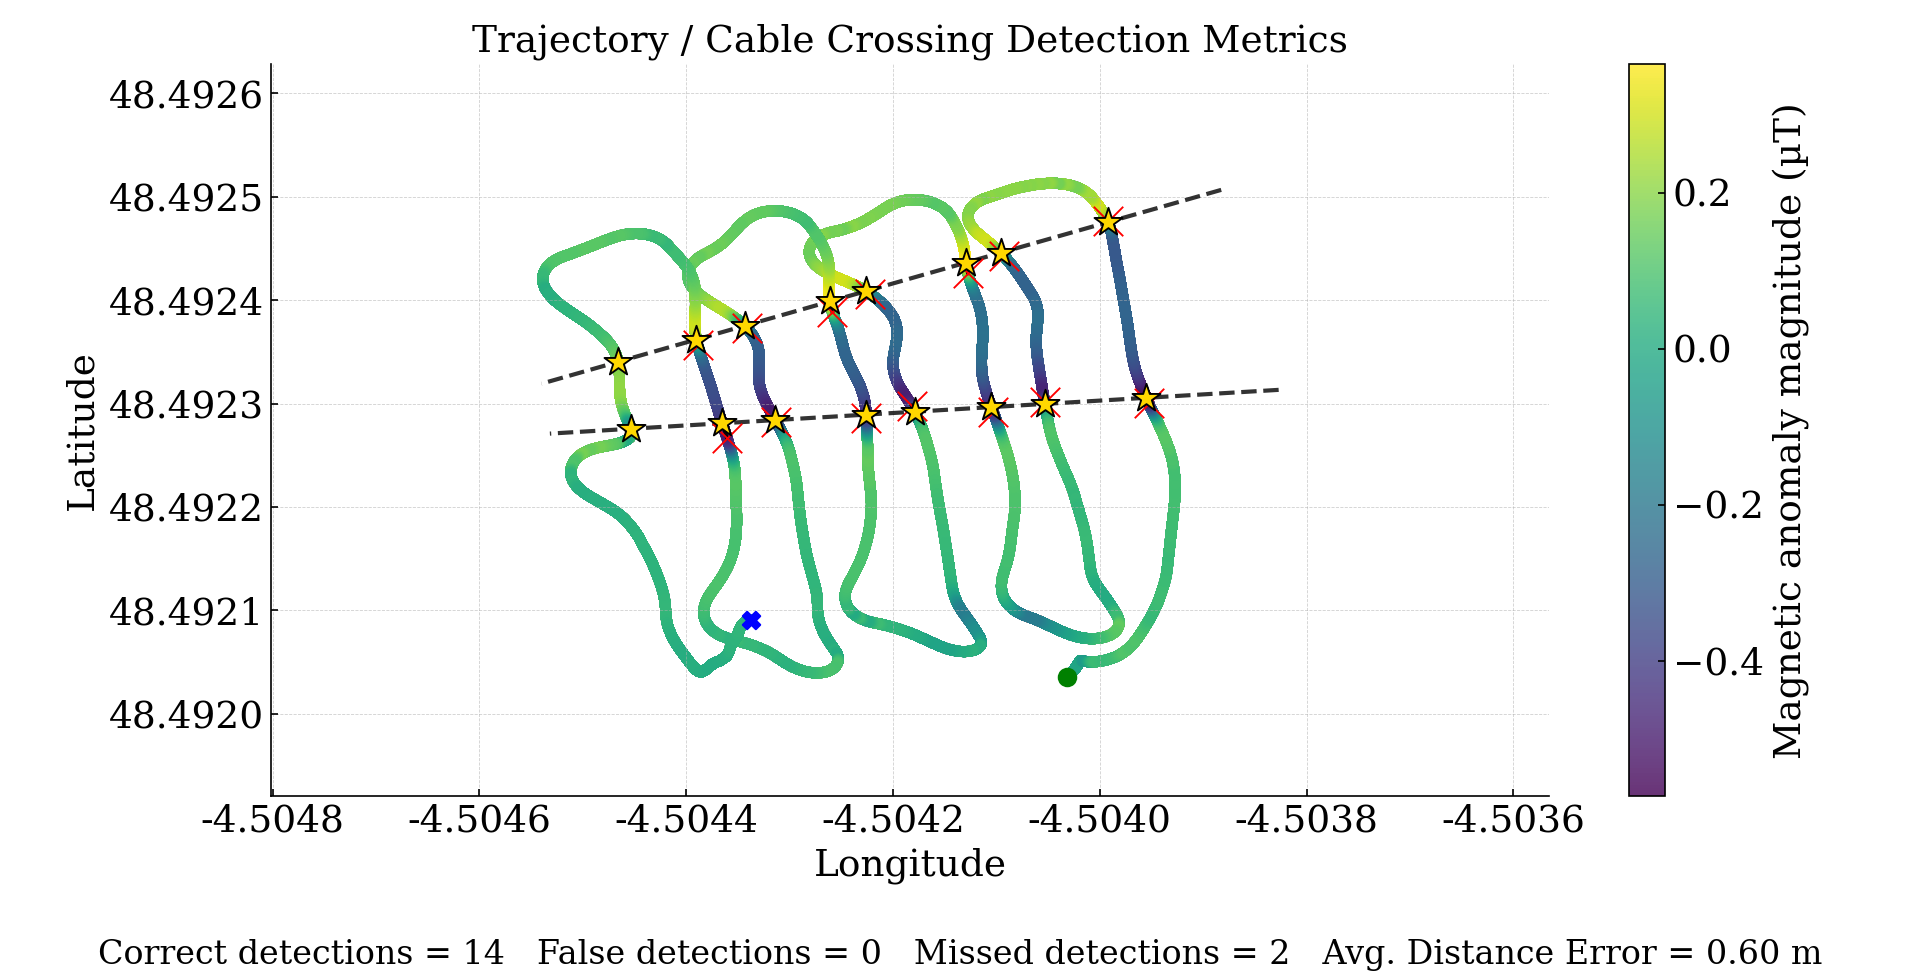
\includegraphics[width=\linewidth]{results_and_discus/figures/trajectory.png}

    MOBF order 1 (Anderson)  
    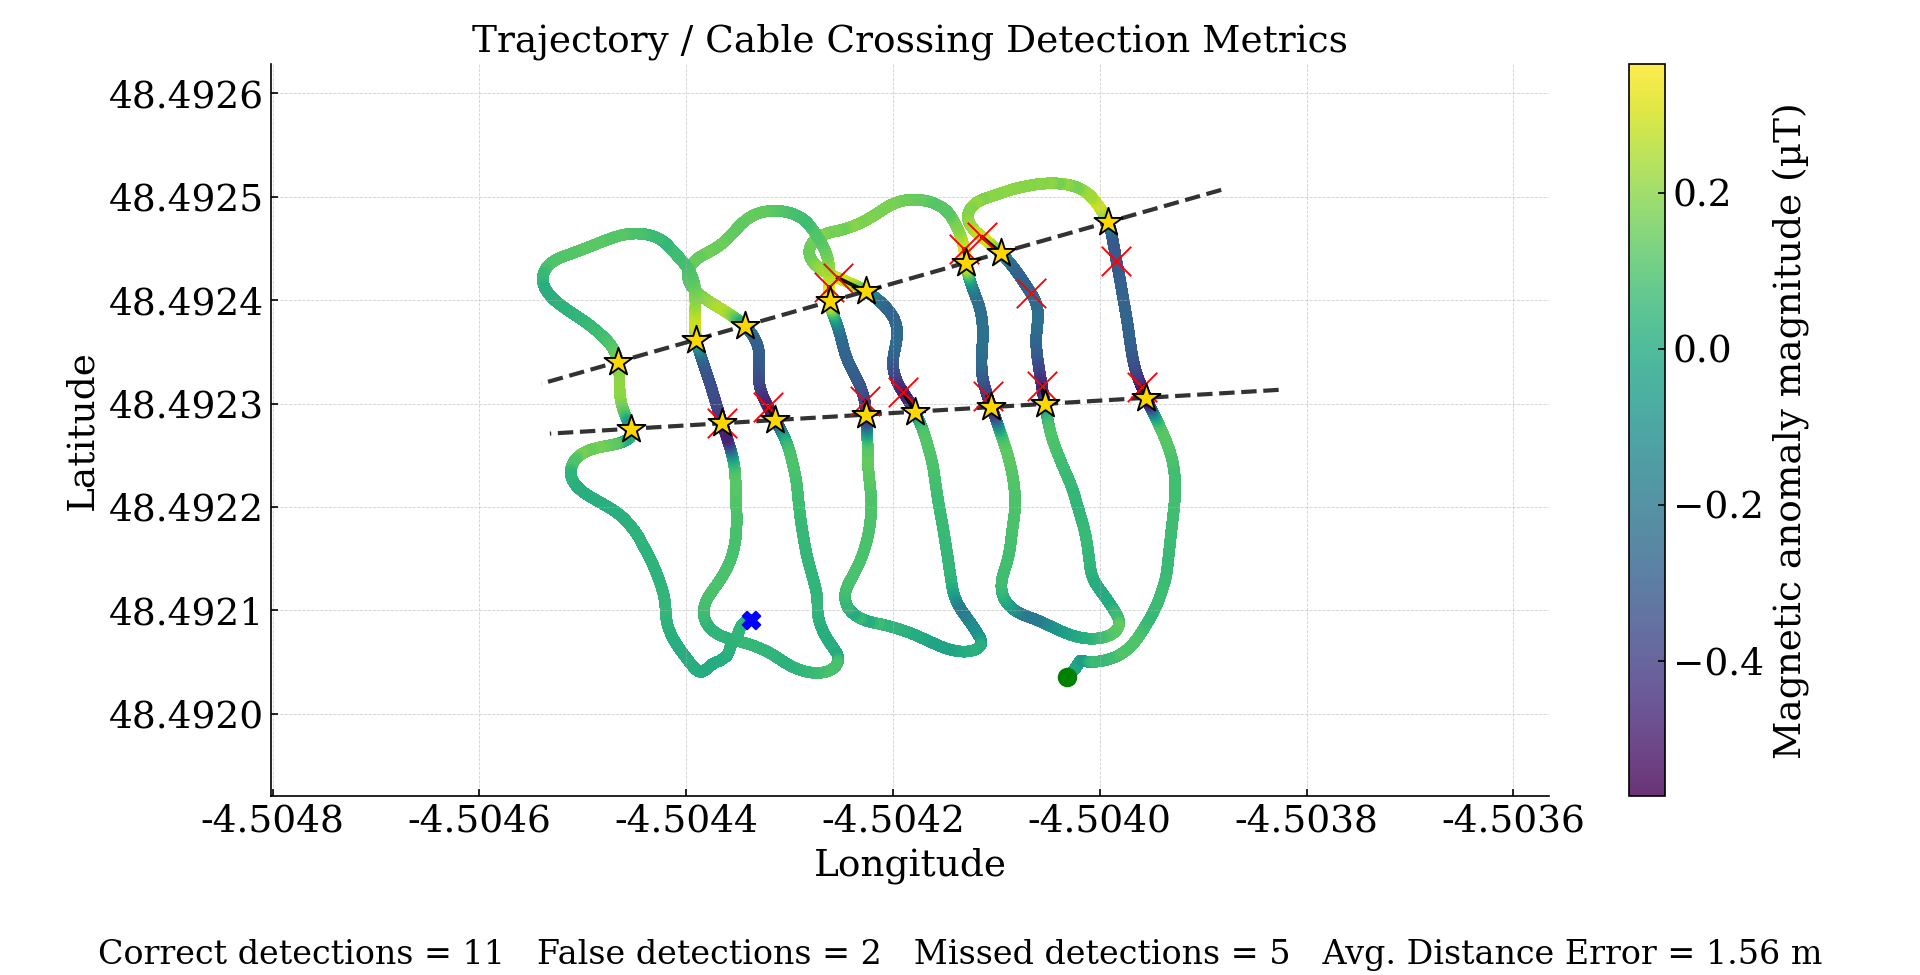
\includegraphics[width=\linewidth]{results_and_discus/figures/trajectoryAnderson.png}

    MOBF order 2 (Quadrupole)    
    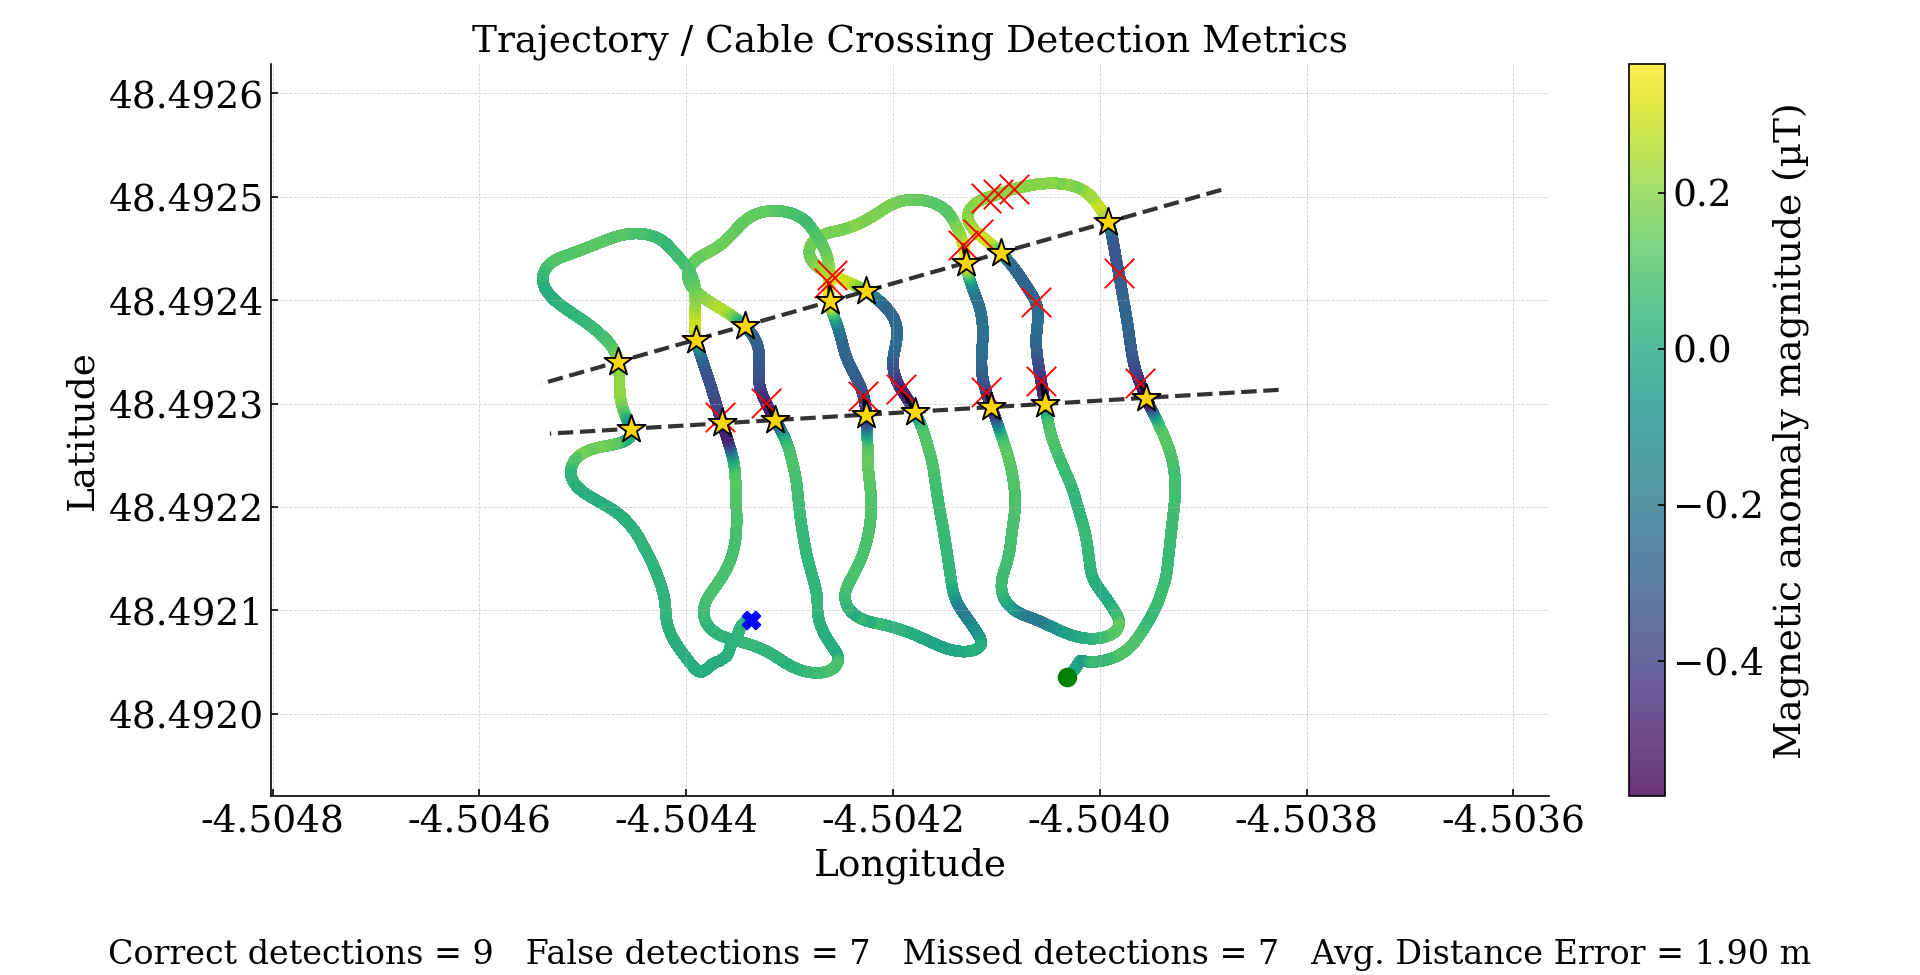
\includegraphics[width=\linewidth]{results_and_discus/figures/trajectoryQuad.png} 

    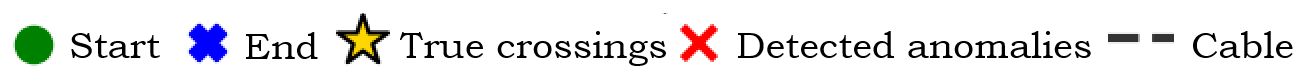
\includegraphics[width=\linewidth]{results_and_discus/figures/trajectory_legends.png}
    \caption{Comparison of detection locations along the USV trajectory relative to the cable position. The color indicates the data entering the filter. Top: detections using the cable OBF. Middle: detections using the dipole OBF. Bottom: detections using the quadrupole MOBF.}
    \label{fig:trajectory_comparison}
\end{figure}

\begin{figure}[ht]
    \centering
    Cable OBF    
    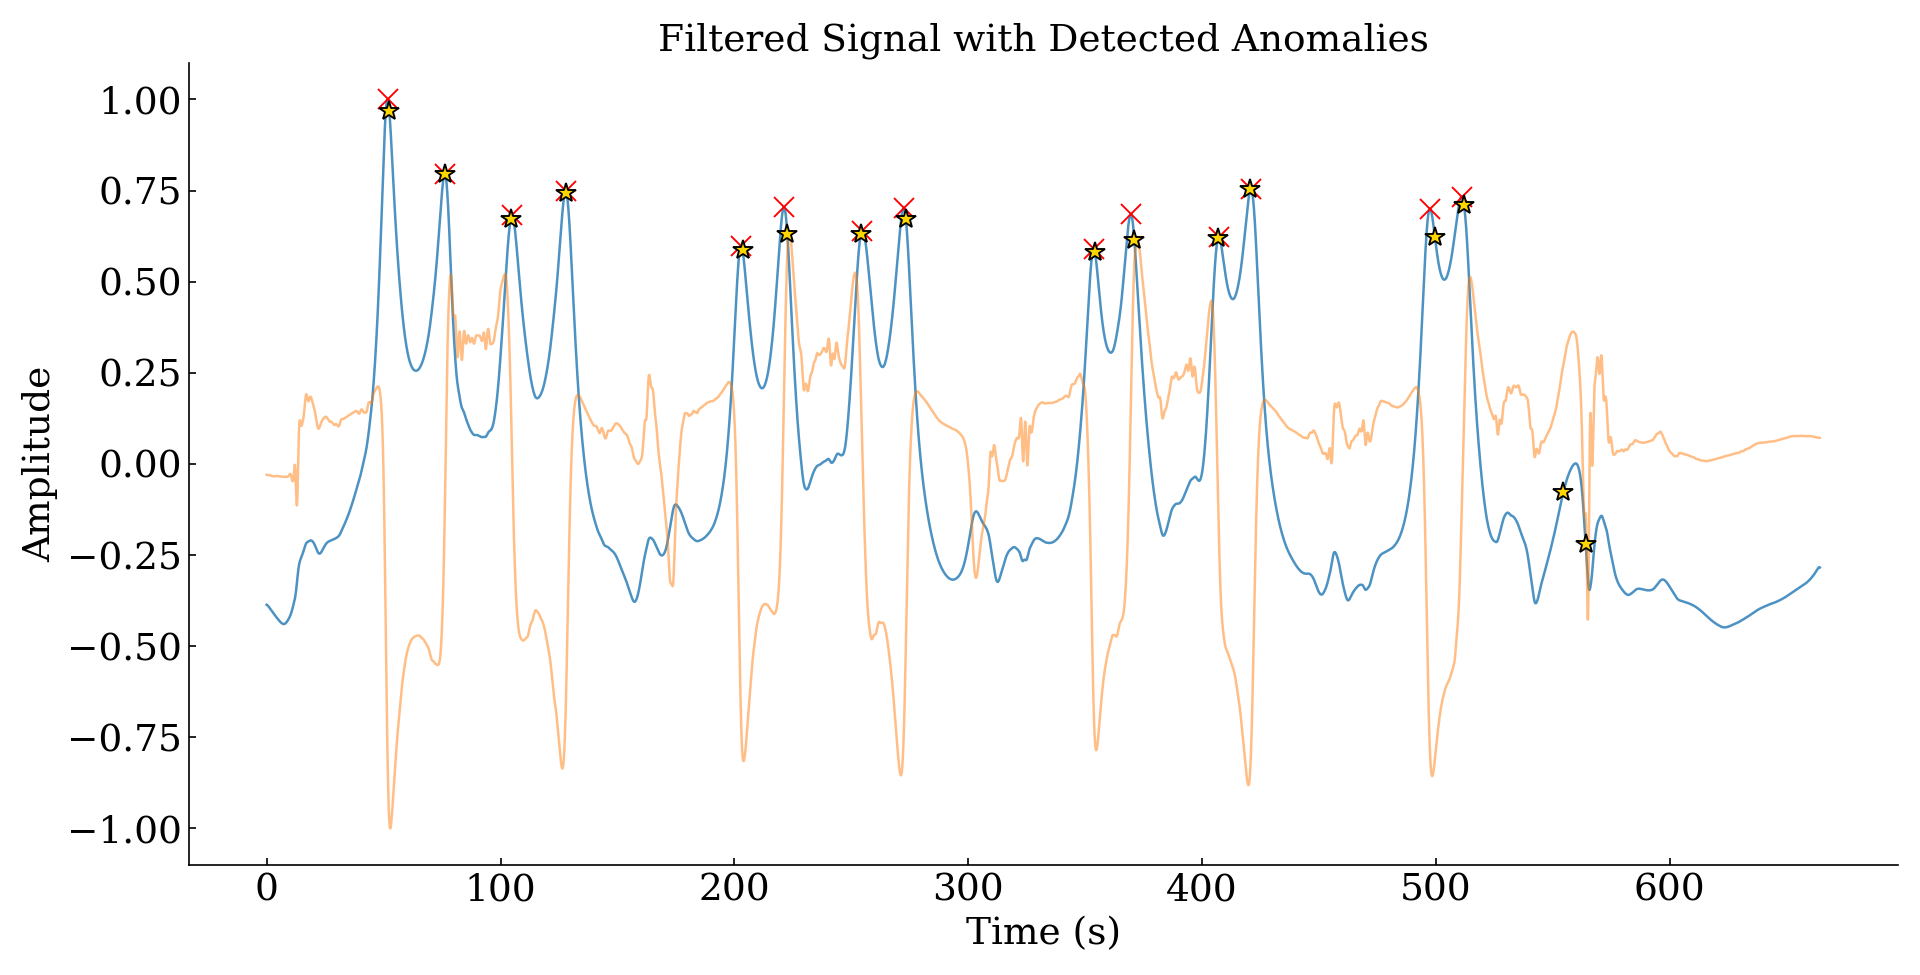
\includegraphics[width=\linewidth]{results_and_discus/figures/filter_output.png}

    
    MOBF order 1 (Anderson)
    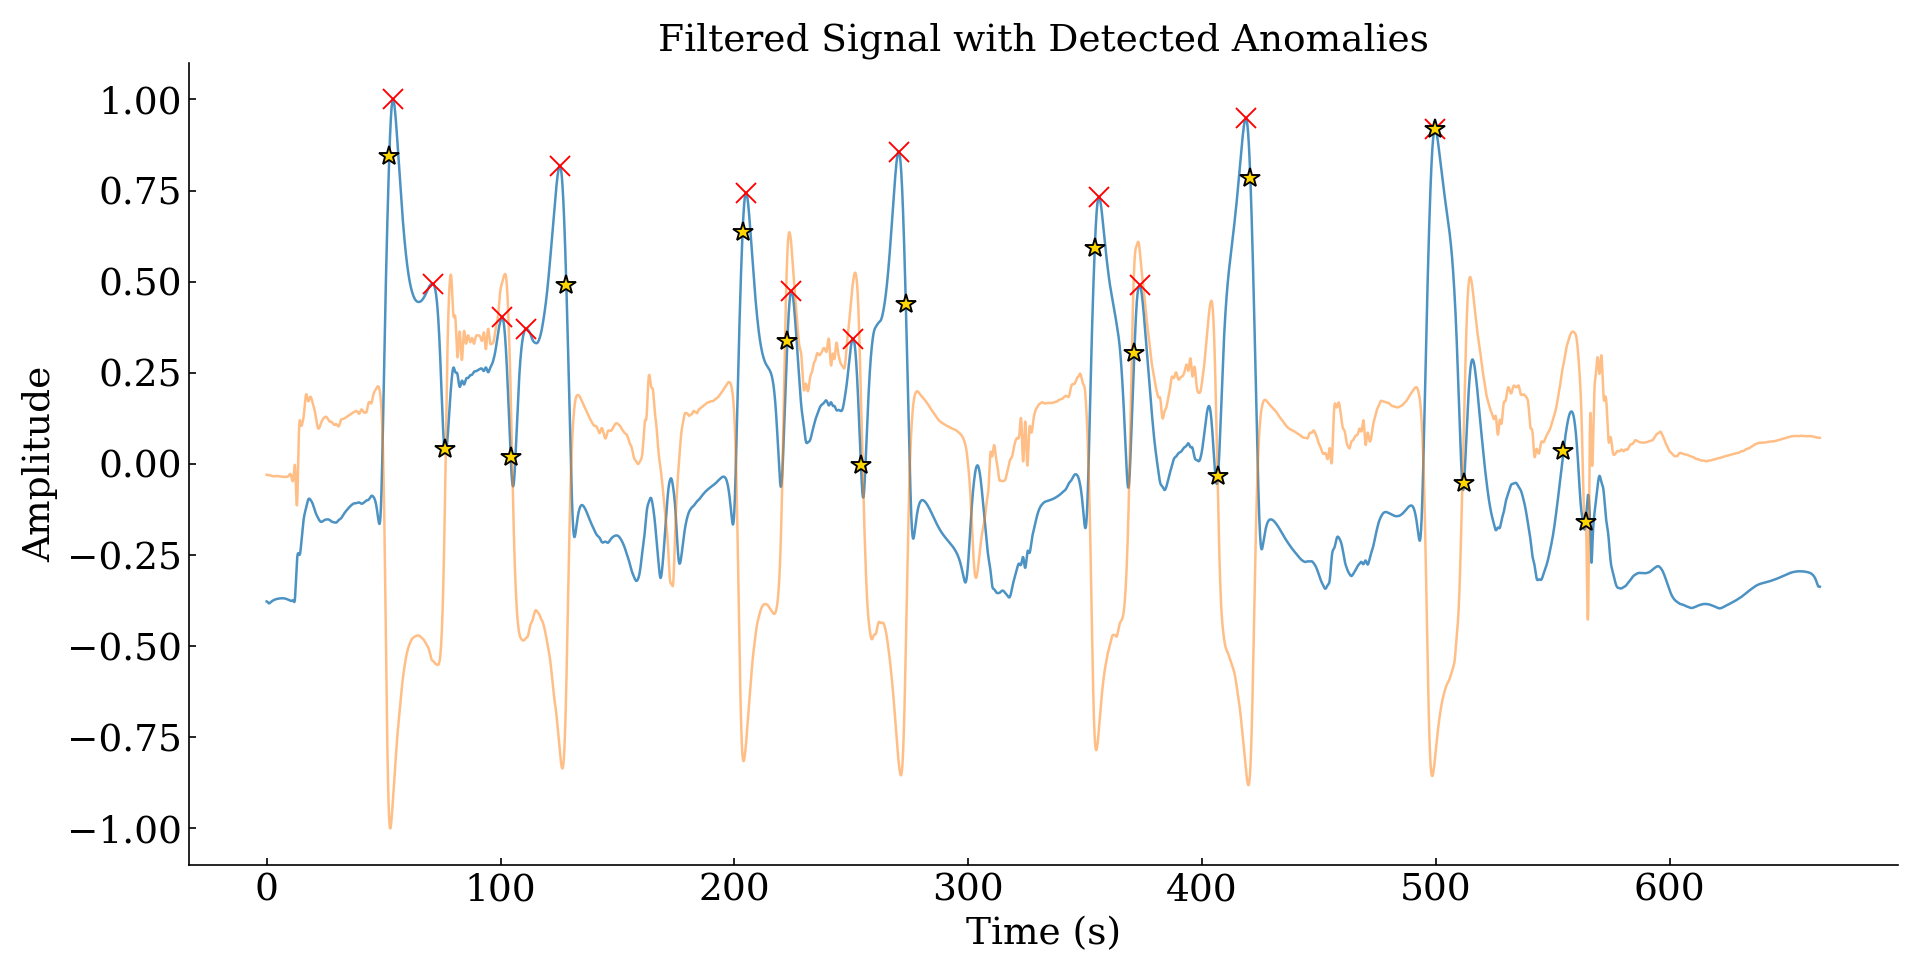
\includegraphics[width=\linewidth]{results_and_discus/figures/filter_outputAnderson.png}
    
    MOBF order 2 (Quadrupole)
    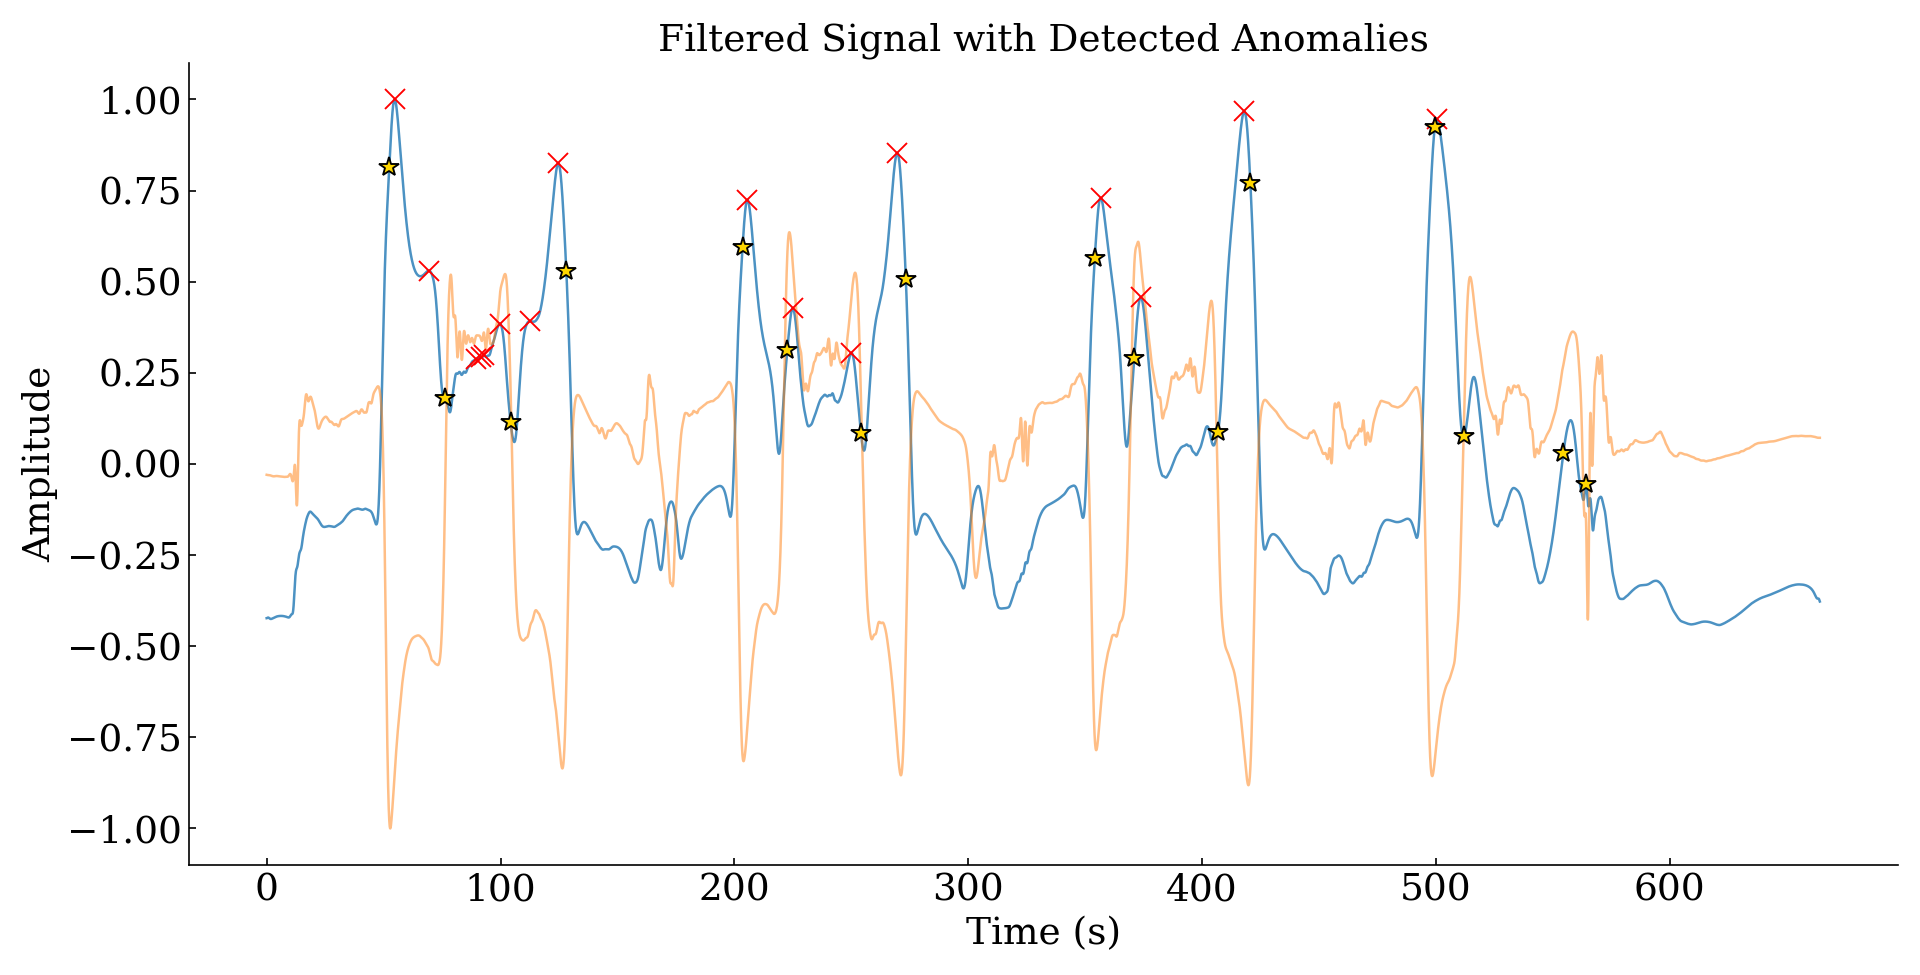
\includegraphics[width=\linewidth]{results_and_discus/figures/filter_outputQuad.png}
    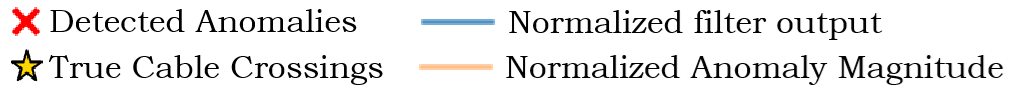
\includegraphics[width=\linewidth]{results_and_discus/figures/filter_output_legends.png}
    \caption{Comparison of filter outputs with detections and true cable crossings. 
    Top: output using the cable OBF. Middle: output using the dipole OBF. Bottom: output using the quadrupole MOBF.}
    \label{fig:filter_output_comparison}
\end{figure}

\subsubsection{Simulation}\label{sec:simulation}

We developed a Python-based simulation framework that produces synthetic trajectories of GNSS coordinates and the corresponding recorded magnetic field for controlled sensor configurations and experimental setups.

Here we simulated the magnetic field of an electric wire following the Biot-Savart law, see equation \ref{eq:mag_field}, and as a trajectory we took a lawnmower pattern with constant velocity $v=1.8~m/s$, the cable depth goes from 1 to 1.5 meters, linearly from start to finish. It carries a DC current of 6A, and the results were mixed with AWGN so that we obtained an SNR of -6dB
\footnote{signal to noise ratio $
\mathrm{SNR}_{\mathrm{dB}}
=
10 \log_{10}\left(
\frac{\sum_t X(t)^2}{\sigma^2}
\right).
$ with $X(t)$ the norm of the recorded magnetic field, and $\sigma^2$ the variance of an AWGN.}.
The simulation was executed at a sampling frequency of 50 Hz, and the same analysis parameters and graphical representations employed in the real experiment were applied here, as illustrated in \autoref{fig:trajectory_comparison_simu}.

Analyzing the plots, we see a similar behavior to that of the real experiment, as our cable OBF, detected the cable presence at the exact moment with so little error (average error of 0.09~meters). The same could not be said for MOBF, as its first order (Anderson), detected the cable with a noticeable lag, leading to a constant localization error of 1.47~meters. A minor observation is that the amplitude exhibits two maxima per crossing. This behavior is most clearly evidenced by the smaller secondary peak around 50~s in Figure \ref{fig:filter_output_comparison_simu} (middle).

In the simulations, the SNR was lower than in the corresponding physical experiments. Under these conditions, the second-order MOBF produced output with increased noise levels and less well-defined peaks, thereby degrading the accuracy and robustness of the localization, giving a better average distance error than the first order (only 0.65~meters), but it is much noisier.

These findings empirically support the superior performance of cable OBF for this study, given that precise and reliable localization constitutes the primary objective of the project.


\begin{figure}[ht]
    \centering
    Cable OBF
    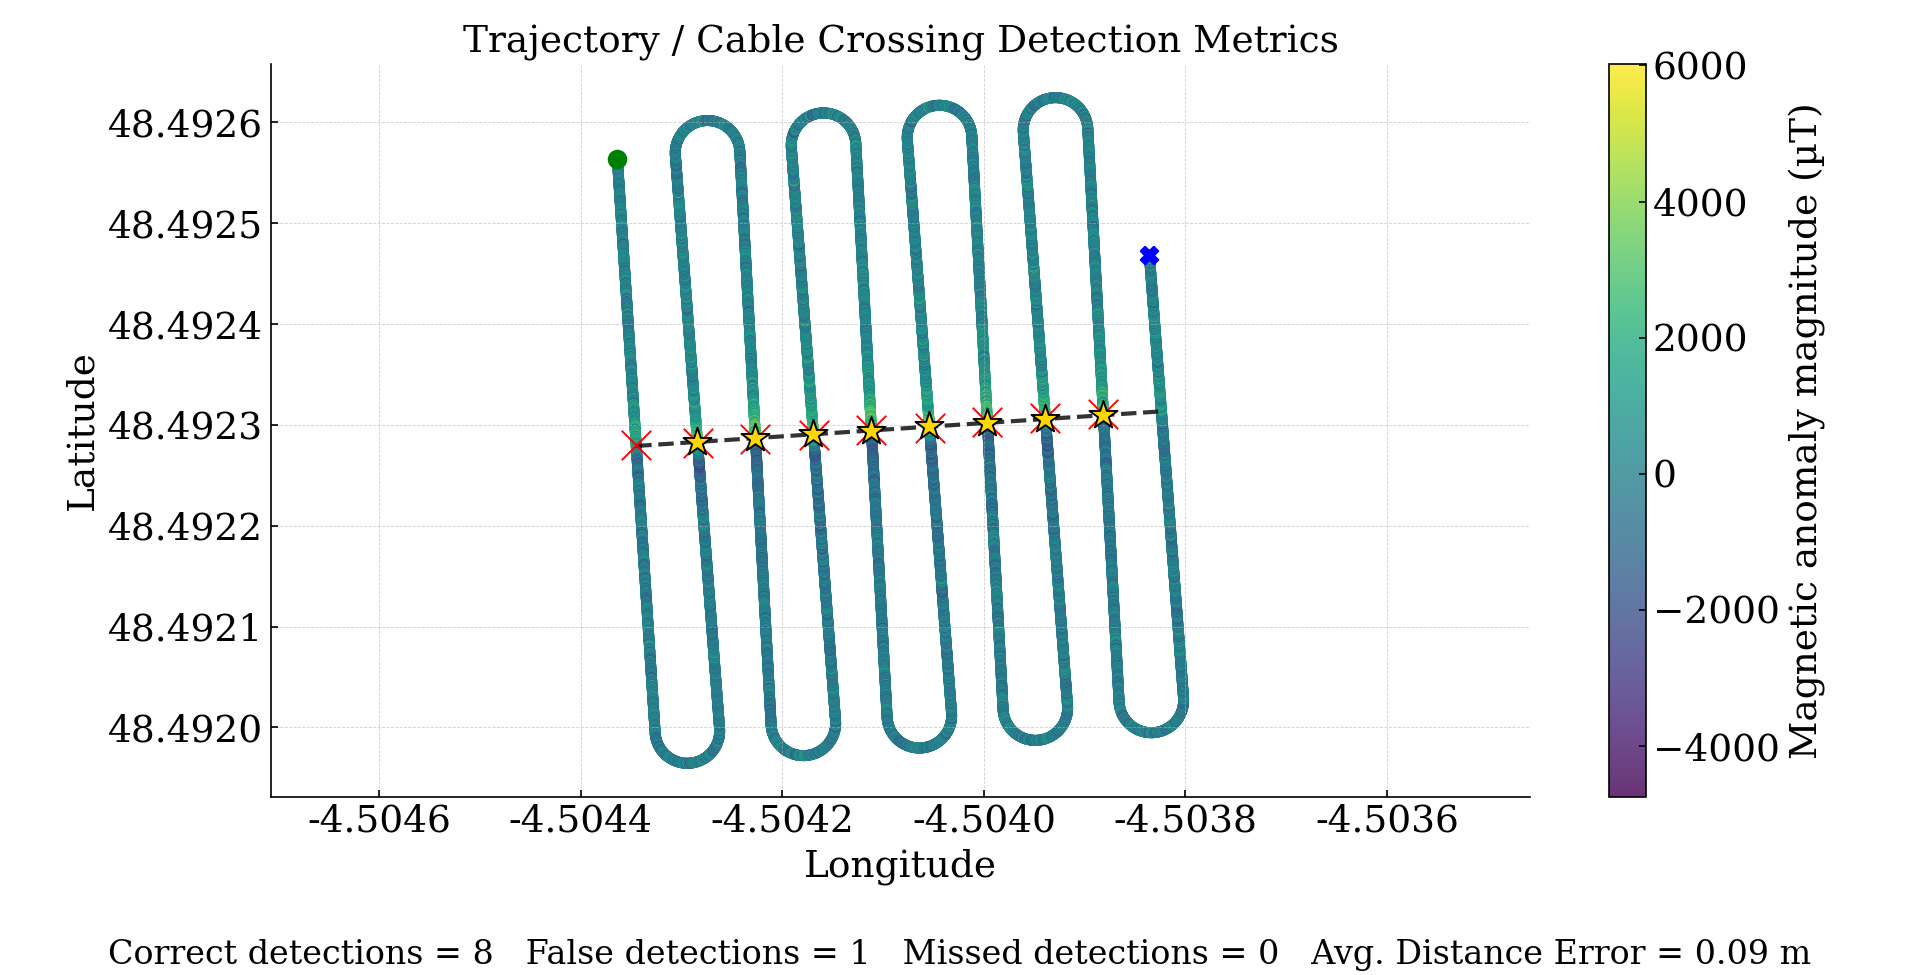
\includegraphics[width=\linewidth]{results_and_discus/figures/trajectory_simu_noisy.png}
    
    MOBF order 1 (Anderson)
    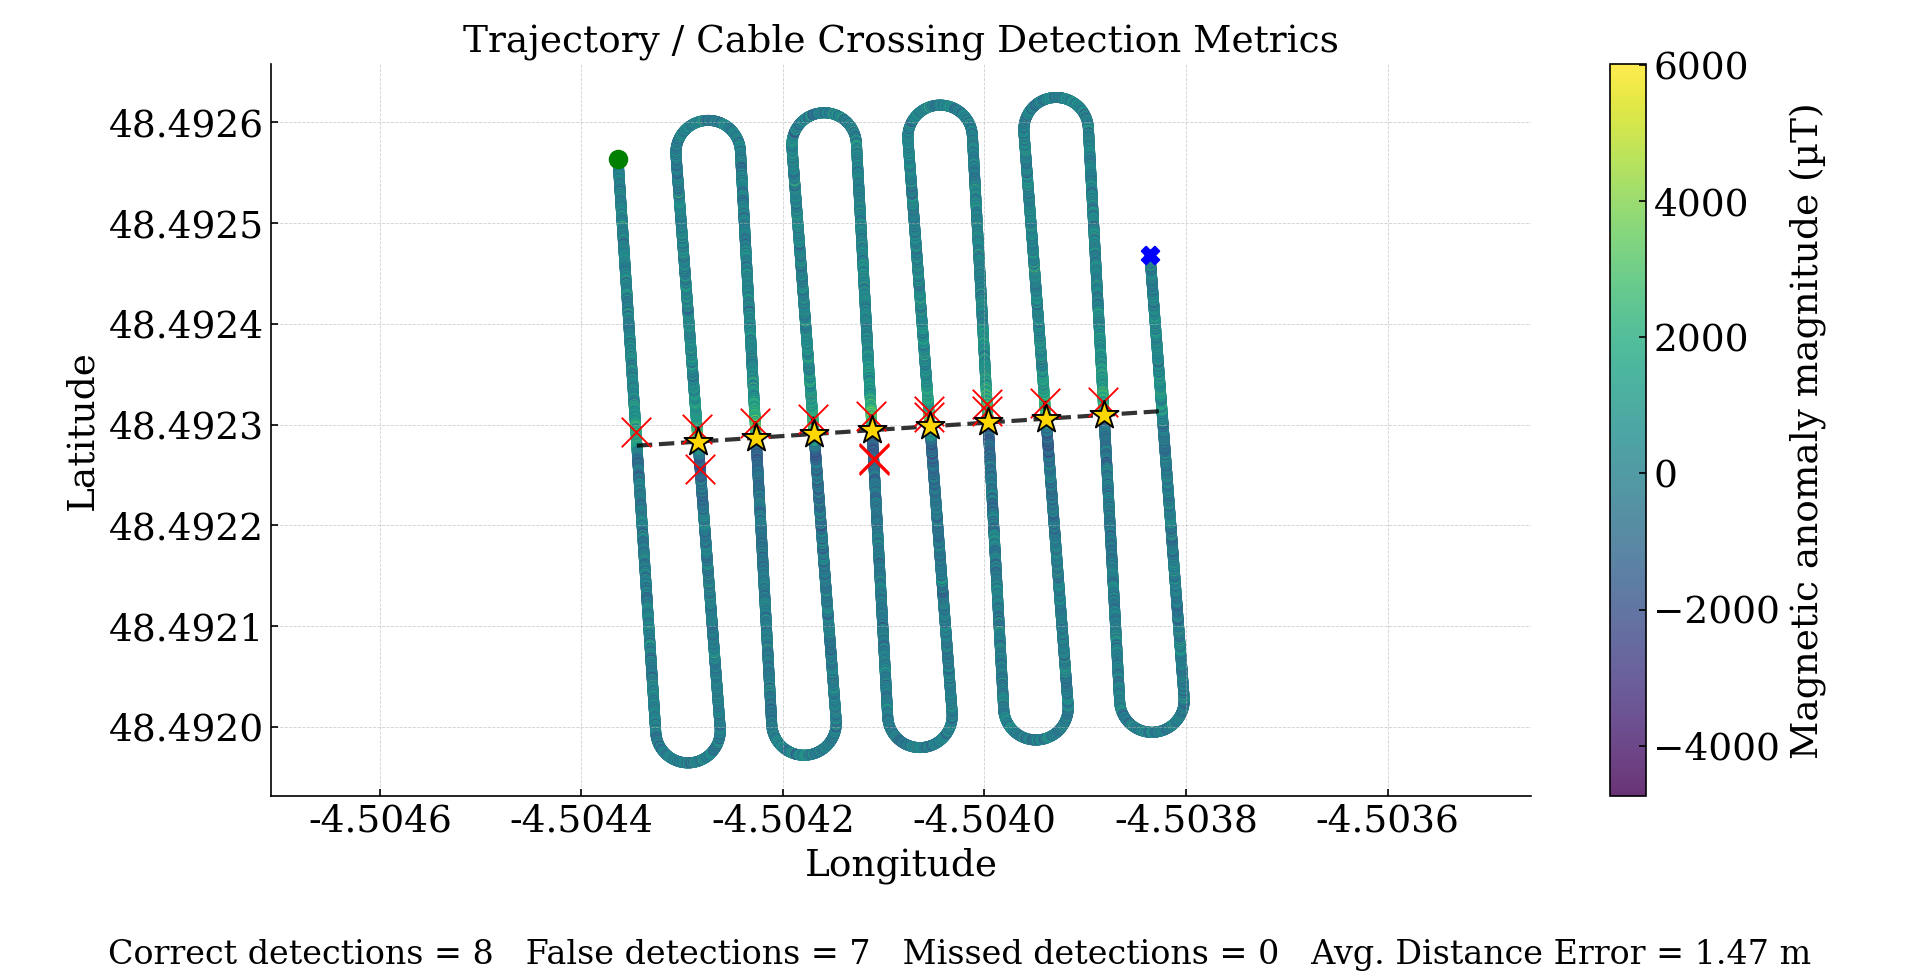
\includegraphics[width=\linewidth]{results_and_discus/figures/trajectoryAnderson_simu_noisy.png}
    
    MOBF order 2 (Quadrupole)
    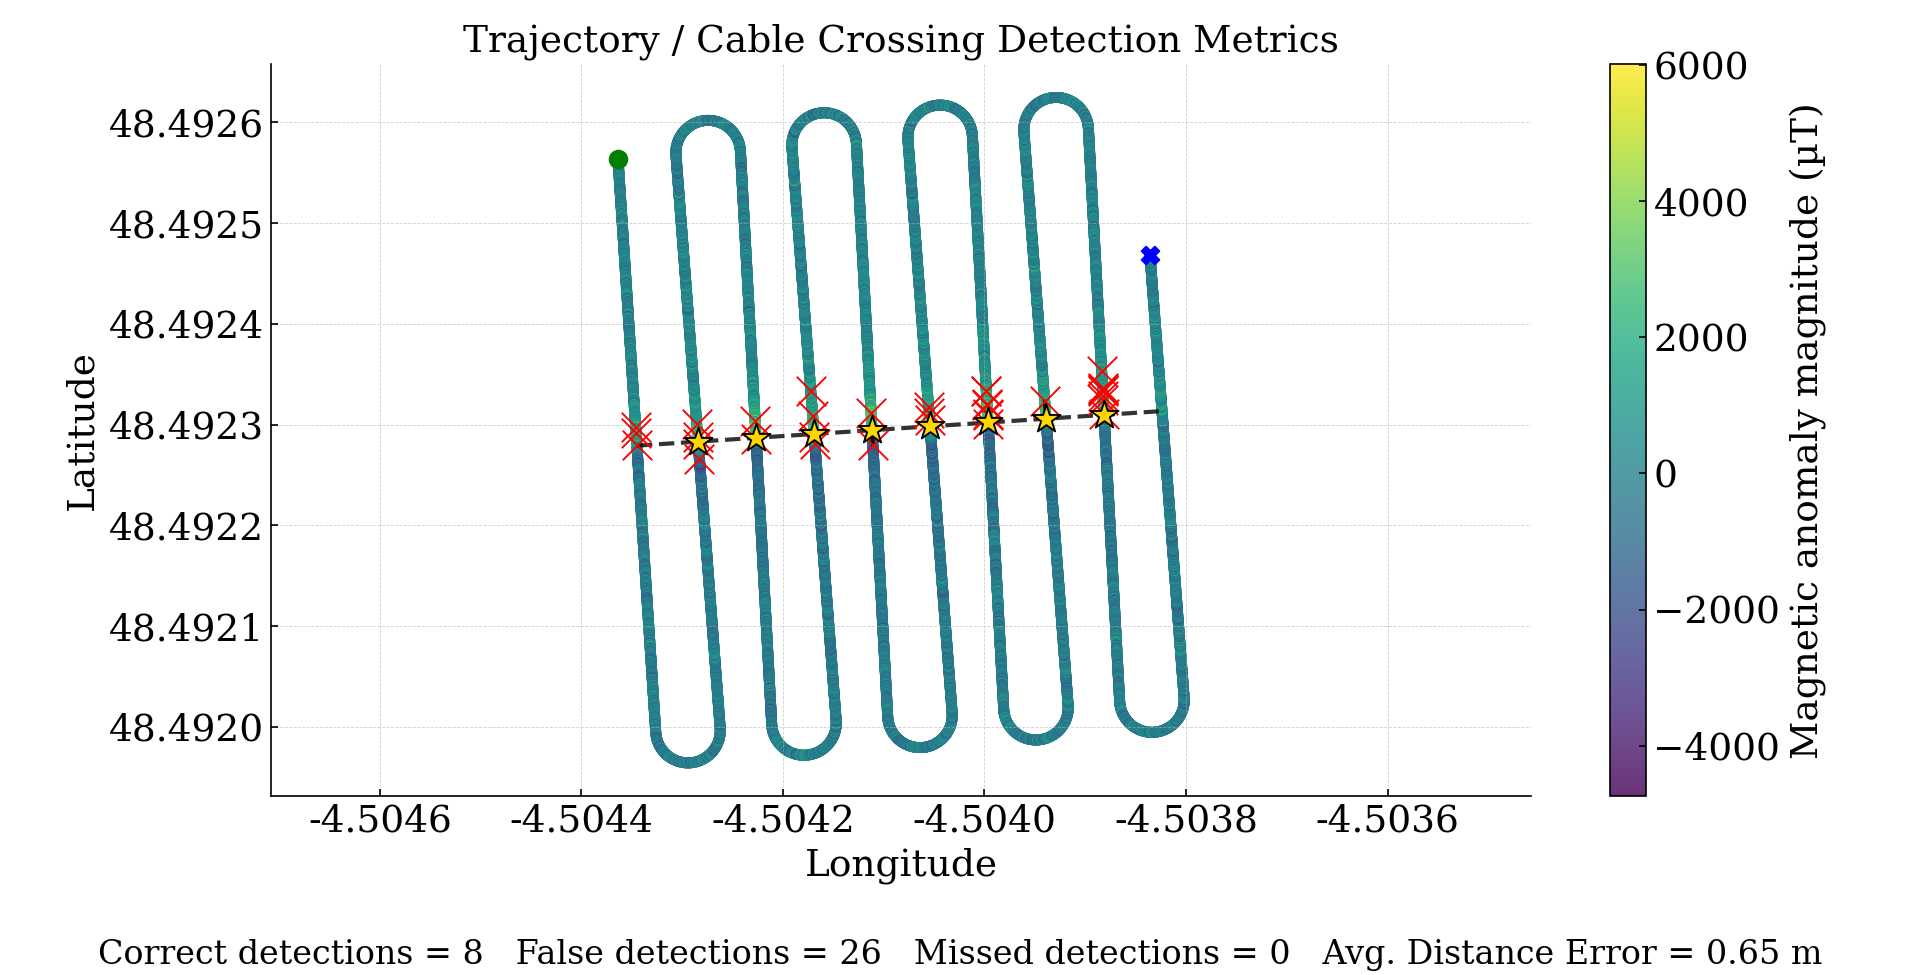
\includegraphics[width=\linewidth]{results_and_discus/figures/trajectoryquad_simu_noisy.png} 
    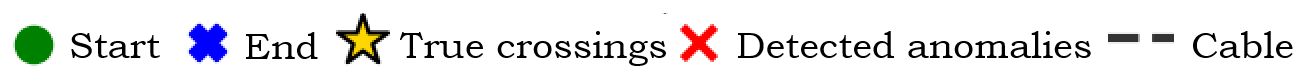
\includegraphics[width=\linewidth]{results_and_discus/figures/trajectory_legends.png}
    \caption{Comparison of detection locations along the USV trajectory relative to the cable position. The color indicates the data entering the filter. Top: detections using the cable OBF. Middle: detections using the dipole OBF. Bottom: detections using the quadrupole MOBF.}
    \label{fig:trajectory_comparison_simu}
\end{figure}

